\section{GALMC}\label{sec:impl}

In this chapter we will present our own implementation of a model checker for Group Announcement Logic called \cname{} and describe its inner workings. \cname{} is intended to be an educational tool which aids students in learning epistemic logic in a more visual manner. Therefore, while most other model checking utilities such as DEMO \cite{JanvanEijck} stick to answering the user's queries with simple yes and no answers, \cname{} goes beyond that by showing them not just whether their formulas hold, but also visualizes why and provides the user with an easier, visual way of drawing models almost as they would on paper or blackboard. The reasoning behind this was that by allowing the user to manipulate the model through a simple click-and-drag interface and seeing how it can affect the valuation of various formulas, they might gain a deeper understanding of the semantics involved.

One of the big questions that needed to be answered when building \cname{} was how to not just present and visualize these highly abstract models, but also allow the user to manipulate them in a way that would be intuitive and easy to grasp. As I had previously used a tool called JFLAP\footnote{www.jflap.org} with great success when teaching students as a TA about Turing machines and finite state automata (FSAs) I ended up drawing most of my inspiration from it when drawing up my initial sketches for how I imagined my own tool might look. While my own experience with JFLAP is mostly limited to visualizing, editing and playing with Turing machines and finite state automatas, it is a fairly sophisticated package of graphical tools covering also covering many other concepts of formal languages and automata theory. JFLAPs editor is relatively simplistic, but it still helped my own and my students' understanding of FSAs tremendously by allowing us to interact and play with what is otherwise a really abstract concept and as such, I wanted to see if I could create a similarly potent learning aid for epistemic logic. 

\begin{figure}[H]
	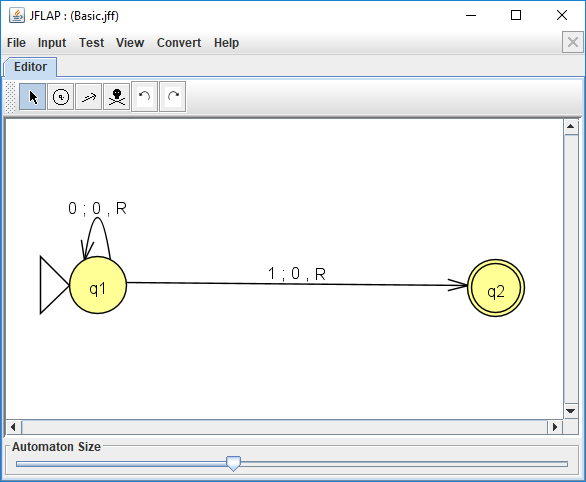
\includegraphics[width= \textwidth]{JFLAPbasicIllustration.PNG}
	\caption{A basic two-state turing machine}
	\label{fig:JFLAP_basic illustration}
\end{figure}

%When I took the same course myself the year before I became a TA in it, most of the students, myself included found Turing machines to be a really hard and abstract concept to grasp as we were simply explained how they worked and then instructed to write instructions that would perform certain basic tasks using pen and paper alone. Obviously, this left us without any way to check whether or not our 

While I could have created a simpler non-graphical model checking tool for GAL similar to DEMO, I wanted to create something more powerful that could help visualize epistemic logic the same way that JFLAP visualizes Turing machines. My justification is that although a similar non-graphical tool would probably have helped me teach my students how FSAs and Turing machines work as well, I highly doubt it would have been anywhere near as effective without being able to visualize the `how's and `why's and instead only gave `yes' or `no' answers to our queries in the same manner that most model checking utilities do. 
%Learning benefit

\subsection{Visualization of Kripke structures}
%Visualization of Turing machines vs kripke stuctures
%Both have states, transitions vs indistinguishability, tape of input vs formula to traverse and check
Although finite state automatons and epistemic logic might initially seem relatively far detached, the Kripke structures we use share a fair few similarities to FSAs that made me realize I could visualize our models in almost the same manner as JFLAP does its automata. For instance, they both consist of a set of states, and while FSAs and Turing machines have transition rules, and Kripke models have an indistinguishability relation, they can both be visualized as edges in a graph where the nodes are our states. Whereas JFLAP labels its edges with the each transition rule, we label ours with the set of agents that considers our pair of states indistinguishable and additionally label each state with the set of propositions that hold in it. We present our tool visualizing a basic model in Figure \ref{fig:basicModelVis}.


\begin{figure}[H]
	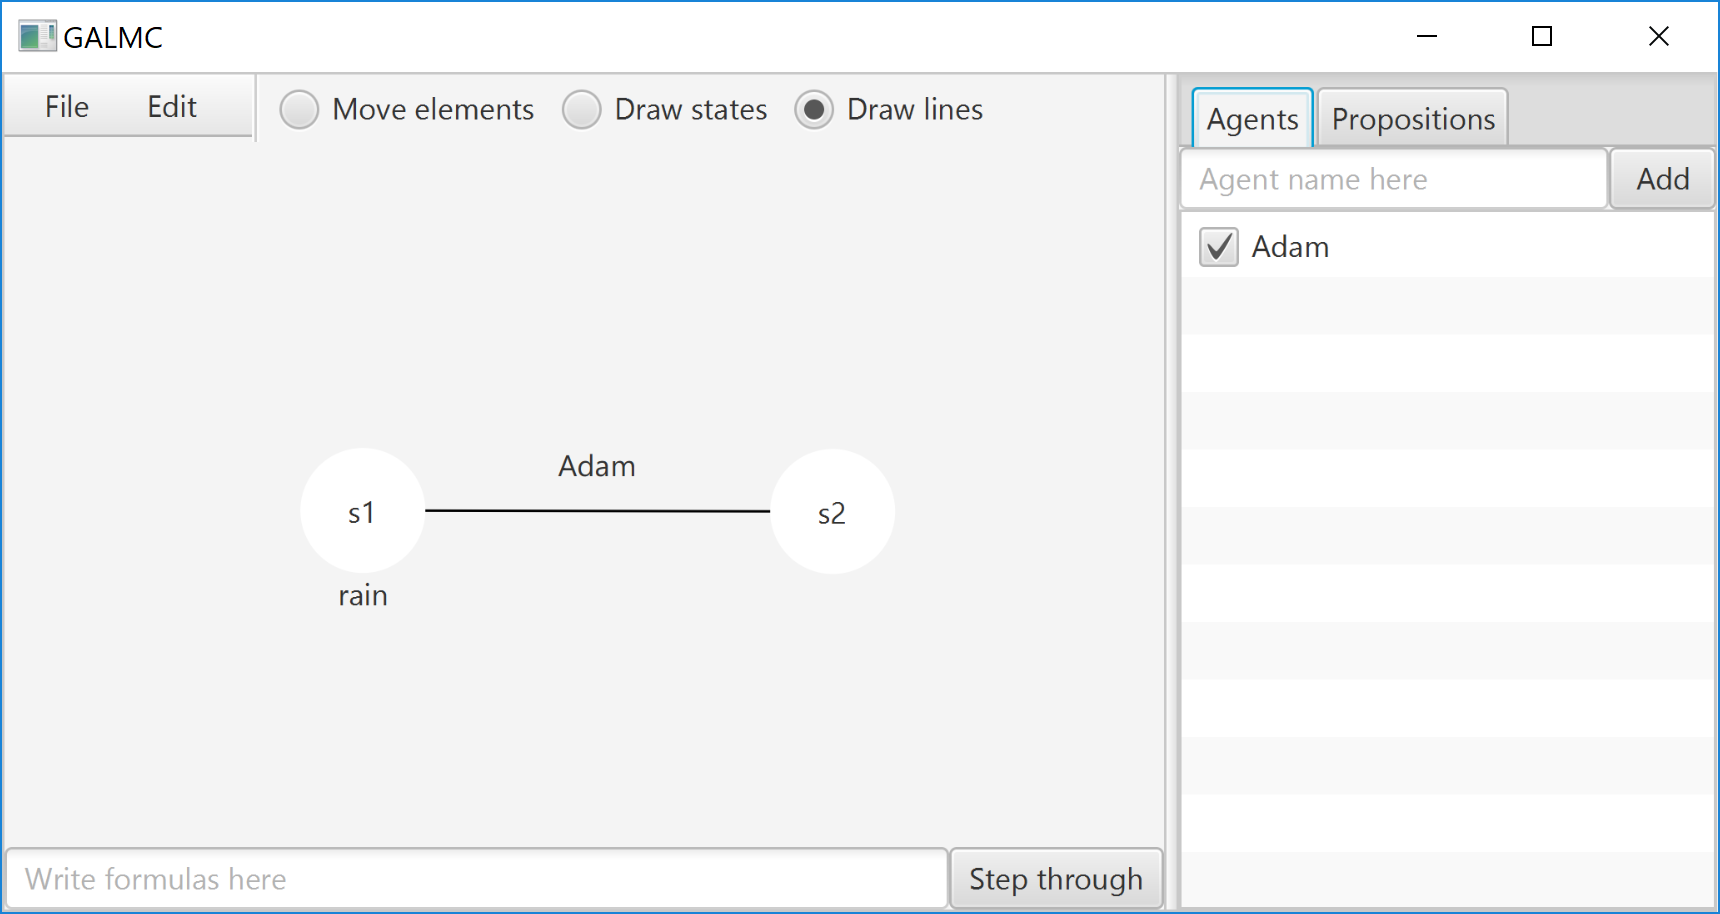
\includegraphics[width= \textwidth]{BasicModel.png}
	\caption{A basic model, visualized in \cname}
	\label{fig:basicModelVis}
\end{figure} 

%Mention basic usage, how one draws models, example blackboard, simple, intuitive, easy
Figure \ref{fig:basicModelVis} shows how \cname{} visualizes the basic model we introduced in Figure \ref{fig:basicEM} and as can be seen, the UI of \cname{} is fairly close to that of JFLAP, in order to capture its simplicity. The reason for this being to enable the user to draw models in a fashion as close to how they would with pen and paper as possible so that the interface feels `natural' and intuitive to someone with little previous experience with Kripke structures. As such, the editor was made to be as clean as possible, consisting of only three main tools; one for selecting and moving elements, one for drawing new states and one for creating edges between them. Additionally, the editor provides two side panels for managing the lists of properties and agents in our models; the proposition panel for selecting which propositions should hold in newly drawn states or to update existing ones, and the agent panel which allows the user to similarly determine which agents' equivalence relations should be updated when manipulating edges.

\subsection{Checking formulas}

After the user creates their model, the next step is to start checking formulas against it. One trade-off that had to be made here was whether or not to stick to the original symbols for the various operators in our language or to come up with replacements which are easier to type in. As most of the logical symbols used to represent the various operators in GAL cannot be found on normal keyboards, naturally making them vary hard for the user to input, \cname{} replaces them with more easily accessible replacements. By the assumption that most of \cname's userbase would be at least somewhat familiar with programming, these replacements were lifted from symbols used to represent boolean operators in programming, such as replacing $\vee$ and $\wedge$ with $|$ and $\&$ for disjunctions and conjunctions respectively, as they can basically be seen as `(inclusive) or' and `and'. A full list of operators and their replacement symbols are displayed in Table \ref{tbl:symbolReplacements}\footnote{This list of replacements and a more complete user guide is also available from https://github.com/AndersKaareEide/MCGAL/wiki}. Note that while announcements are identical to how they are in GAL, the curly braces around the set of agents in group announcements were dropped to save the user the effort of typing them in. The knowledge operator is fairly similar, except that \cname{} forces agent names to start with an upper-case letter and that the parentheses around the known formula are required. The reason behind these changes was partly to be able to make it easier for the user to tell names of agents apart from propositions in more complex formulas (\cname{} forces agent names to be capitalized, whereas propositions have to be lower case). That said, the editor translates any formula the user types in back into proper legal formulas when displaying them, making it easier for the user to connect \cname's representations with other material.

%the tool less confusing to use, once the user gets familiar with the tool and the logic itself \footnote{For a more to the point user manual, see: https://github.com/AndersKaareEide/MCGAL/wiki}.

% Uppercase agent name, easier to tell props from agents?
% but it also ended up making the parser a lot simpler to write, which will be presented and discussed a later section

\begin{table}[H]
\centering
%\resizebox{\textwidth}{!}{%
\begin{tabular}{@{}lcc@{}}
\toprule
Operator           & Logical symbol & Replacement     \\  \midrule
Negation           &       $\neg$         & !               \\
Conjunction       &      $\wedge$          & $\&$              \\
Disjunction        &    $\vee$        & $|$               \\
Implication        &       $\rightarrow$       & -\textgreater{} \\
Knowledge         &        $K_{ann}\varphi$        & $KAnn(\varphi)$            \\
Announcement   &       $[\varphi]\psi$         &  $[\varphi]\psi$     \\
Group Announcement &  $[\{ann,bob\}]\varphi$  & $[Ann,Bob]\varphi$ \\ \bottomrule
\end{tabular}%
%}
\caption{Table of operators and their symbols in \cname{}}
\label{tbl:symbolReplacements}
\end{table}

%Include BNF as table? Save it for ANTLR section

%Checking formulas, visualize which states in our model satisfy the given formula
%Mention interactive formula display with subformulas

When the user finishes typing in their formula, the tool checks their formula against each state in their model and colors each state based on whether or not the user's formula is satisfied in that state. However, in addition to translating the user's input into a legal formula and showing which states of the model satisfy the formula, \cname{} also lets the user hover over parts of their original formula in order to check the valuation of its subformulas, which can be seen in Figure \ref{fig:labelHover} (Note the mouse cursor over the `clouds' proposition). This enables the user to quickly break formulas apart and see how their various subformulas change the valuation of their containing formula. It also helps visualize the semantics behind each operator in our language in a manner that makes the logic more enjoyable to learn. 

\begin{figure}[H]
	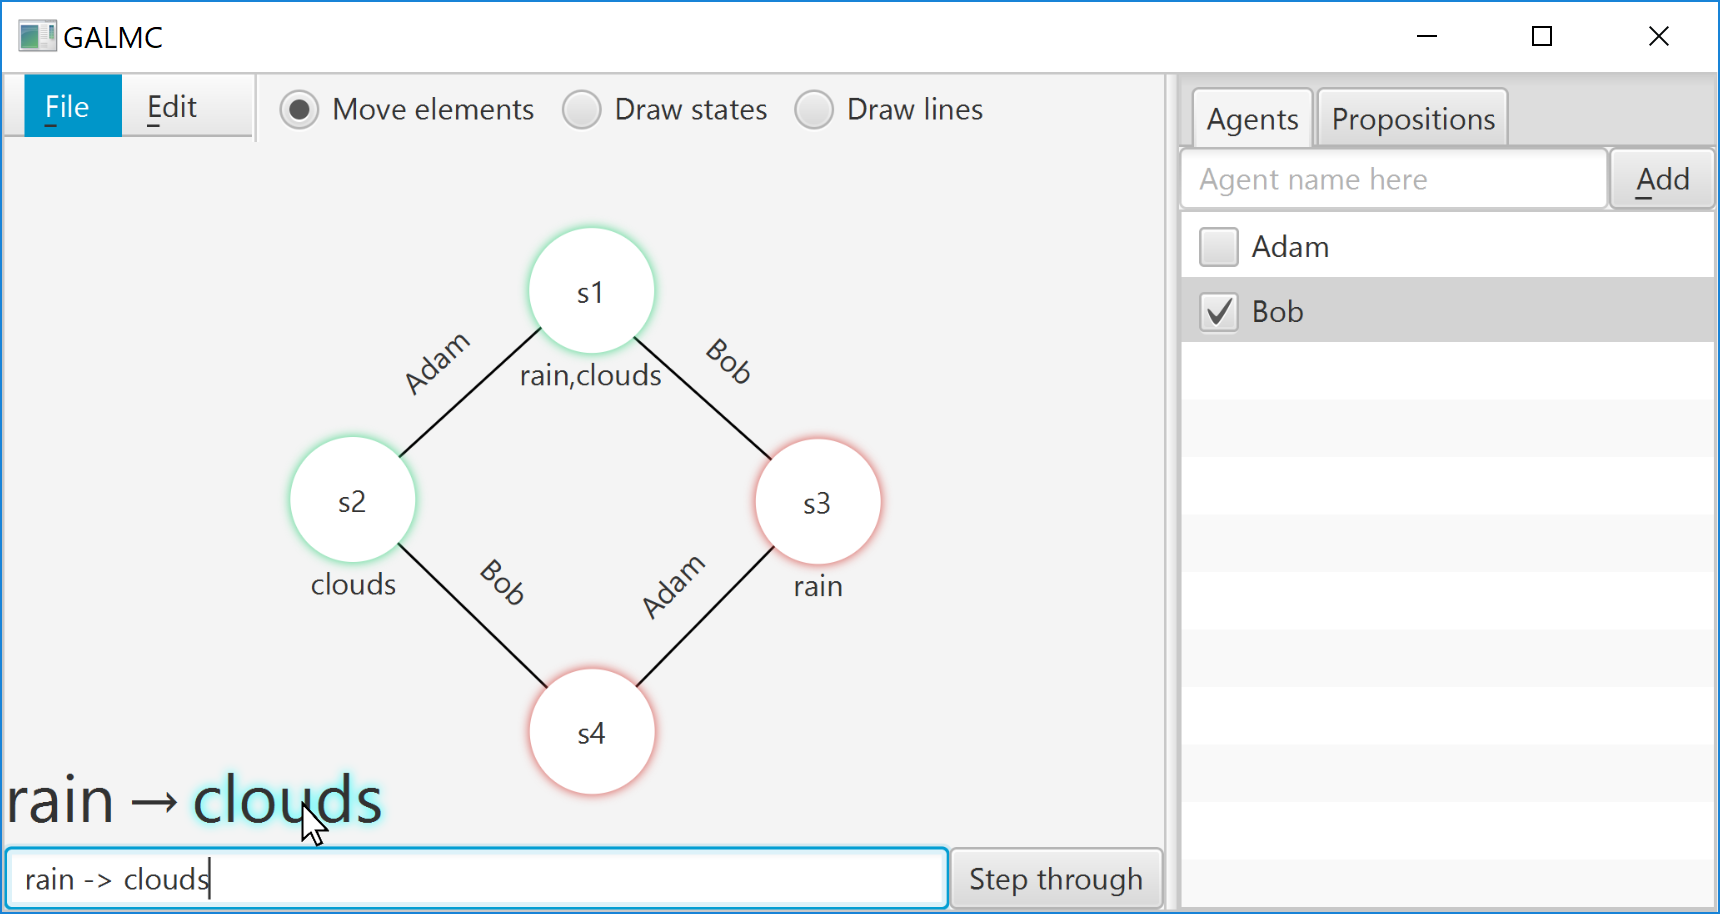
\includegraphics[width= \textwidth]{LabelMouseOver.png}
	\caption{Illustration of mousing over interactive formula display}	
	\label{fig:labelHover}
\end{figure}


\subsection{Visualizing the checking process}

One of JFLAP's most powerful features however, is its ability to step through your automatons. As you present your Turing machines in JFLAP with a set of input, the tool also allows you to step through the program of your machine one instruction at a time, while also visualizing how it manipulates the contents of its input and which state the machine is currently in. Obviously this feature is remarkably useful in showing how the user's machines operate, letting students debug their instruction sets in almost the same manner they would debug a program in a high level programming language. As such, it not only makes Turing machines and FSAs much easier to grasp, but it also makes getting them to work correctly a far less frustrating process.

Naturally, \cname{} having a similar feature, a way to visualize the process behind checking each operator in the user's formula the same way that JFLAP shows each instruction being executed and the effects of doing so would greatly improve its usefulness. This is why the tool keeps a log of each check the tool makes when evaluating a formula, logging not just the operator being checked, but also its current valuation, if known, and which state it is being checked in. Continuing with the model from our previous figure, Figure \ref{fig:stepperBasic} shows us using our tool to generate a log of how the program checks the given formula against a specific state. From this, the user can get a fully reproducible guide they can follow when checking other formulas on their own, which would be quite helpful in learning how the operators work. The user can also step forwards or backwards through this process at any time by either clicking the step they want to skip to, or browsing with the arrow keys. 

Note that in addition to this log, the program also visualizes which (sub)formulas are being checked against the various states as colorized labels that change color as the user steps through their formula based on the valuation of the operators the labels represent. 

\begin{figure}[H]
	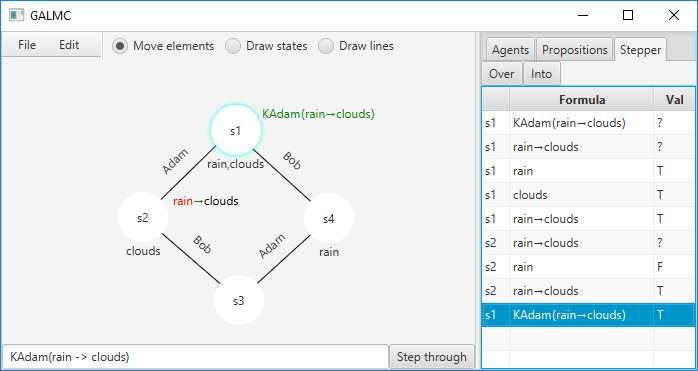
\includegraphics[width= \textwidth]{SteppingBasicExample.png}
	\caption{Illustration of using stepping functionality in \cname{}}
	\label{fig:stepperBasic}
\end{figure}


Returning to our previous comparison between the stepper in JFLAP and our adaptation for GAL, there is still an interesting challenge. While the instruction sets and states of a Turing machine are static, the epistemic models we use in dynamic epistemic logic are naturally quite dynamic, and can be updated based on public announcements in PAL or more complexly, group announcements in GAL. \cname{} represents these model updates by graying out the states and edges that were removed by the update and to update which states should be `hidden' based on which branch in the tree-like structure of the original formula the user is currently stepping through. Naturally, the tool also supports formulas with multiple announcements nesting them in any fashion the language allows, always visualizing the relevant sub-model that formulas are being checked against, an example of which can be seen in Figure \ref{fig:stepperUpdates}. Note that \cname{} also generates formula labels for which subformulas under knowledge or announcement operators have been checked in the various states, so that the user can immediately see why for example, an agent does not know something, or why a state has been filtered out in a model update.

\begin{figure}[H]
	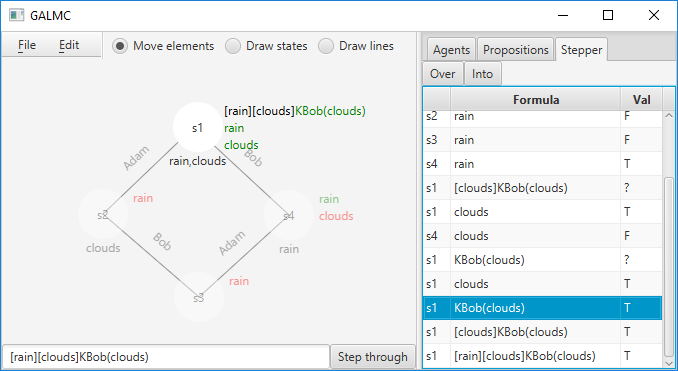
\includegraphics[width= \textwidth]{SteppingChainedAnnouncements.png}
	\caption{Visualization of the effects of chained public announcements in \cname{}}
	\label{fig:stepperUpdates}
\end{figure}
 

%Innholdsliste:

	%	Likheter i stepping over teip med input vs stepping over operatorer i formel, vise endringer i valuering i 'sanntid' på samme måte som teipen til JFLAP 
%Vis mer avansert eksempel med public announcements og modell-oppdateringer
%Vis eksempel med group announcements og hvordan verktøyet visualiserer de ulike strukturene koalisjoner kan begrense den orginale modellen til
	%	Muligens visualisere kunnskap de dicto vs de re? Må finne enkelt eksempel som ikke blir horribelt rotete i så fall


%Mention deviation from logic here? Flipped valuation function, 

\subsection{Visualizing group announcements}

Now that I have presented most of the tool I have created and how it solves the various challenges of visualizing the process of checking formulas containing the other operators in our language, it is time to discuss group announcements. As the motivation behind creating \cname{} was to create a learning tool that could help new logicians understand how the semantics of GAL work, being able to generate examples which highlight interesting properties of our models is highly important. As such, \cname{} was designed from the ground up to be able to trace its steps through the model checking process so that it can also display each step of this process in an intuitive manner, which can be seen in our previous figures. Elaborating on the logging process mentioned before behind this tracing, the tool also keeps track of subformulas and formula depth as it goes through the operators. The reason behind keeping track of this in the logs was to create a more easily navigable tree-like structure, as the number of steps required to check a formula containing group announcements can quickly explode. Because of this, \cname{} must give the user the ability to skip through chunks of the process they might not be particularly interested in. This tree-structure allows them to for example view each state the tool checks against a particular knowledge operator, or even skip through each of the possible updated models a coalition can reduce a model to through their announceable extensions, without having to step through the checking of the inner formula every time. 
 
\begin{figure}[]
	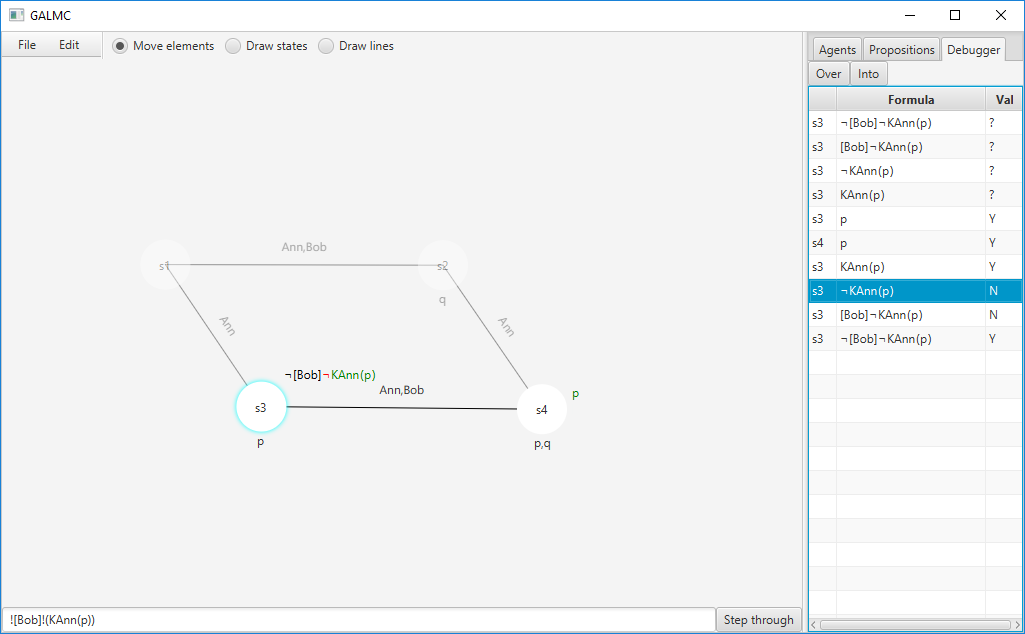
\includegraphics[width= \textwidth]{MCGALBasicChecking.png}
	\caption{Checking a basic group announcement formula in MCGAL}
	\label{fig:basicGalChecking}
\end{figure}

%\todo{Flette inn med resten av det over}

As the tool provides a view of the model and keeps track of what the model it is currently checking against looks like, it can also visualize the effects of announcing multiple different formulas. This means the tool can also visualize the result of constraining the model to the various formula extensions a coalition can announce, which is what is being displayed in Figure \ref{fig:basicGalChecking}. In this example, we are checking whether the formula $\neg [Bob]\neg K_{Ann}[p]$ holds in state s3 of our model. The formula roughly translates to: `It is not the case that Bob is unable to make Ann know $p$' or more simply in its dual form: `Bob is able to make Ann know p'. From the visualization of our model in Figure \ref{fig:basicGalChecking} we can see that since Bob is able to reduce the model to only states where $p$ holds, Ann also knows that $p$ holds in this updated model, satisfying our original formula. In this simple illustrative example, the tool ended up only having to try announcing a single formula extension before it found an extension that made our original formula true. If we were to check a more complex formula however, it might end up checking many different announcements, each generating a different updated model after its announcement which the tool will helpfully visualize, giving the user insight into a coalition's capabilities. 

%Note that the previous example could also have been made easier by rewriting the formula as $\dia{Bob}K_{Ann}[p]$, but unfortunately the tool does not (yet) support diamond operators. 

Last, but certainly not least, \cname{} also facilitates saving and loading of models. As our tool is intended to be used in educational settings, making lecturers able to create exercises for their students is highly valuable. One example of such usage would be creating and handing out an incomplete model, where the students would have to `complete' the model by either adding states or changing the indistinguishability relations for their agents in order to give this model some specific property. The lecturer could then load the models that their students have handed in to verify them. 

%As I used a similar approach to great success when introducing JFLAP to my students while teaching them automata theory and turing machines, I know how useful this feature can be. As such I wanted to make sure that my own tool could be used the same way.

%Saving / loading, distribuering av eksempler
%Oppgaver som kan gis ut, delvise modeller som skal fullføres av studenter og leveres inn

%Figure \ref{fig:debugExmpl} shows a screenshot of \cname{} in action, where the user is stepping through the process of checking a specific formula against a state in their model, having the tool visualize whether or not their formula holds. It also shows how the application breaks down epistemic formulas into sub-formulas and displays them next to each state they have to be checked in. Additionally, the application also visualizes the current valuation of each operator and proposition in the formula as you step through the checking process, as can be seen from the red and green parts of the formulas being checked, as well as the Val (valuation) column in the debugger tab. 

%Something something easier to show if we supported formula templates, future work
%Highlight difference between being able to achieve something and knowing that you are able to achieve something


%* Discuss how formulas are interpreted / parsed into tree-structures where each the nodes themselves 'contain' definitions for the semantics behind the logical connective they represent, based on their class.
%* Refer back to previously presented algorithms when discussing recursive checking function
%* Refer back to background chapter when discussing why the problem is interesting when presenting artifact.
%* Model checking often limited to yes / no questions, discuss added value by transcending boolean 

%JFLAP, a tool previously used here at our faculty to teach students how turing machines and finite state automatas work.


%Splitte opp i delkapitler? Sjekking av EL, sjekking av DEL, sjekking av GAL?

%Innholdsliste:

%Recap motivasjon
%Forklar hvorfor grensesnittet ble som det ble, inspirasjon fra JFLAP ect
%Anekdote rundt bruken av JFLAP 
	%Nytte for studenter
%Introduksjon til visualisering, vis basics
	%Trekke sammenligninger mellom visualiseringen av Kripke og FSAer
%Diskuter tegning av modeller, tilstander, kanter og agenter
	%Grunngi tegnemåte og andre avgjørelser iht UI, sidepaneler, editor-'moduser'
%Nevn håndtering av props og agentlister

%Vis eksempler på sjekking av basic formler
%Forklar innlesing av formler
%Diskuter forskjeller mellom innskreven form vs logiske symboler (enklere å skrive inn)
%Forklar hva som skjer, først sjekk hvilke states i modellen
%Nevn interaktivitet gjennom sjekke subformler ved å muse over

%Diskuter motivasjon og hensikt bak stepping-funksjonalitet
	%	Sammenlign med stepper i JFLAP
	%	Mer avansert enn JFLAP, FSA samme sett states, DEL har modelloppdateringer, kan visualiseres
	%	Likheter i stepping over teip med input vs stepping over operatorer i formel, vise endringer i valuering i 'sanntid' på samme måte som teipen til JFLAP 
%Vis basic eksempel på hvordan verktøyet presenterer steg-loggen
%Vis mer avansert eksempel med public announcements og modell-oppdateringer
%Vis eksempel med group announcements og hvordan verktøyet visualiserer de ulike strukturene koalisjoner kan begrense den orginale modellen til
	%	Muligens visualisere kunnskap de dicto vs de re? Må finne enkelt eksempel som ikke blir horribelt rotete i så fall

